% HomeworkSolutions.tex
% by Erin Kiley <emkiley at mcla dot edu>
% May 18, 2014
% This file is licensed under a Creative Commons Attribution-ShareAlike 3.0 United States License ( https://creativecommons.org/licenses/by-sa/3.0/us/ )
% 
% Sample homework solutions

\documentclass[letterpaper,10pt]{article}

\usepackage{simplemargins,enumitem,amssymb,amsmath,verbatim}
\setallmargins{0.5in}
\setbottommargin{1in}

% Mathy commands
\providecommand{\abs}[1]{\left\vert{#1}\right\vert}
\providecommand{\dabs}[1]{\abs{\abs{#1}}}
\providecommand{\inv}[1]{{#1}^{-1}}
\providecommand{\code}[1]{\fvset{frame=single,numbers=left, numbersep=3pt}\VerbatimInput{#1}}
\providecommand{\st}{\ensuremath{\;:\;}}
\providecommand{\D}{\ensuremath{\;\mathrm{d}}}
\providecommand{\eps}{\ensuremath{\varepsilon}}
\providecommand{\Rn}{\ensuremath{{\mathbb{R}^n}}}
\providecommand{\R}{\ensuremath{{\mathbb{R}}}}
\providecommand{\Z}{\ensuremath{{\mathbb{Z}}}}

\providecommand{\sol}[1]{\vskip0.5em
\fbox{\begin{minipage}{0.9\textwidth}
\noindent{\textbf{Solution.}}
#1
\end{minipage}}\vskip0.5em
}

% Plotting commands
\usepackage{pgfplots}% Uses tikz
\pgfplotsset{compat=newest}% use newest version

\tikzset{My Line Style/.style={smooth, thick, samples=400}}

\begin{document}
\noindent Calculus I\\
\noindent E1 Term, Sections E101 and E196\\
\noindent Instructor: E.M.\ Kiley\\
\noindent May 18, 2014

\begin{center}\textbf{Week 1: Solutions to Written Homework Problems}\end{center}

\begin{enumerate}[label=\textbf{Problem \arabic*.}]

\item 
	\begin{enumerate}[label=\textbf{(\alph*)}]
	\item An oil field containing 50 wells has been producing 10,000 barrels of oil daily. For each new well that is drilled, the daily production of each well decreases by 2 barrels per day. Write the total daily production $P$ of the oil field as a function $P=f(x)$ of the number $x$ of new wells drilled, and clearly explain your reasoning.

\sol{
\begin{equation*}\begin{split}
P=f(x)&=(\text{total \# of wells after new ones are drilled})(\text{daily production per well})\\
&=(50+x)\left(\frac{10,000}{50}-2x\right)\\
&=(50+x)(200-2x)\\
&=-2x^2+100x+10,000.
\end{split}\end{equation*}
}

	\item What are the independent and dependent variables of $f$, and what are their units?

\sol{
The independent variable of $f$ is $x$, the number of new wells to be drilled. The dependent variable is $P$, the number of barrels of oil per day that the field produces.
}
	
	\item State the domain of $f$ as a mathematical function, and state the domain of $f$ that is practically relevant to the scenario being modelled. Explain why these differ.

\sol{
The domain of $f$ as a mathematical function is all real numbers, and this can be written either: $D=\mathbb{R}$ or $D=(-\infty,\infty)$.\\

The domain of $f$ as a practical modelling tool must exclude negative numbers, because the problem didn't entail taking away any wells that already exist in the field. It also must exclude non-integers, because it would be impossible to drill a non-integer number of new wells. We write this either: $D=\{x\in\mathbb{Z}:x\geq0\}$, or $D=[0,+\infty)\cap\mathbb{Z}$. Please look up the concept of set intersection if you wish to use the proper interval notation for a problem like this.
}

\pagebreak
	\item Use the technique called ``Completing the Square''\footnote{If you need a refresher on this, see \texttt{http://en.wikipedia.org/wiki/Completing\_the\_square\#Overview}} to get $f$ into a form whose graph you can draw using the technique described on Page 18 of the text. Draw the graph of $f$, including all labels, arrows, and axis markings.
	
\sol{We use the formulas derived in Lecture 1, namely---if we want to write the quadratic equation $y=ax^2+bx+c$ in the form $y-k=a(x-h)^2$, then the second equation uses the same value of $a$ as the first, and it uses values of $h$ and $k$ that are computed according to:
\begin{equation*}
h=-\frac{b}{2a},\qquad k=c-\frac{b^2}{2a}.
\end{equation*}
For us, we want to convert the equation $y=-2x^2+100x+10,000$ into the form $y-k=a(x-h)^2$, and so we substitute the values $a=-2$, $b=100$, and $c=10,000$ into the formulas to obtain:
\begin{equation*}
h=-\frac{100}{2(-2)}=25,\qquad k=10,000-\frac{100^2}{2(-2)}=11,250.
\end{equation*}

From this, we can use the following information to construct the graph:
\begin{itemize}
\item The parabola opens downward ($a$ is negative);
\item The parabola is relatively ``skinnier'' than $y=x^2$ (because $\abs{a}=2>1$);
\item The vertex of the parabola is at $(h,k)=(25,11250)$;
\item The zeros of the parabola are at $x=-50$ and at $x=100$ (because the original equation we found was in factored form $y=(x+50)(-2x+200)$).
\end{itemize}

The graph of the function looks as follows:

\pgfmathdeclarefunction{SolutionX}{1}{%
    \pgfmathparse{\x}}
\pgfmathdeclarefunction{SolutionY}{1}{%
    \pgfmathparse{-2*\x^2+100*\x+10000}}


\begin{center}
\begin{tikzpicture}
\begin{axis}[
	axis lines=middle,
	xmin=-70, xmax = 120,
	ymin=-1000, ymax = 12000,
	xlabel={$x$}, ylabel={$P$},
	minor x tick num = {2},
	minor y tick num = {2},
	scaled ticks=false,
	yticklabel style={
		anchor = east,
		/pgf/number format/precision=0,
		/pgf/number format/fixed,
		/pgf/number format/fixed zerofill,
	},
]
    \addplot[My Line Style, color=black,  variable=\x, domain=-70:120] 
        ({SolutionX(\x)},{SolutionY(\x)});
    \addplot+[
   		mark=*,
		/tikz/fill=black,
		/tikz/color=black,
		/tikz/draw=black,
		/tikz/mark size={2.5},
		point meta=explicit symbolic,
		] coordinates {(25,11250) [(25,11250)]};
\end{axis}
\end{tikzpicture}
\end{center}
}	
	
	\item Determine the maximum daily production $P_\text{max}$ of the oil field, and $x_\text{max}$, the number of additional wells that should be drilled in order to produce that maximum daily output. Show these values on the graph you drew for part (c).
	
\sol{We determine the maximum daily production by inspecting the graph. It should be apparent that the maximum value on this downward-opening parabola is its vertex, and we thus find that $(P_\text{max},x_\text{max})=(25,11250)$. Please see this red dot plotted on the graph above.
}

\pagebreak
	
	\item State the range of $f$, using both set notation and interval notation. Remember that the range of output values of a function generally depends on the domain to which that function's input values are restricted. Do the two different domains you found in part (c) also correspond to different ranges of $f$?
	
\sol{
The range of $f$ as a mathematical function is
\begin{equation*}
R=(-\infty,11250],\text{ or }R=\{P\in\R\st P\leq11,250\}.
\end{equation*}
This is apparent from looking at the graph, but it is also apparent from looking at the function, since for $P$ in the stated range, we can always find at least one $x\in\R$ such that $P=-2x^2+100x+10,000$. To \emph{find} this (these) $x$-value(s), we use the familiar quadratic formula
\begin{equation*}
x=\frac{-b\pm\sqrt{b^2-4ac}}{2a}=\frac{-100\pm\sqrt{100^2-4(-2)(10,000-P)}}{2(-2)}=25\mp\frac{1}{2}\sqrt{22,500-2P}
\end{equation*}

The two different domains that we found in part (c) do correspond to different ranges of $f$; in particular, since our common-sense restriction was to limit the domain to non-negative integers, the output range will be different as well. In particular, this domain can be written conveniently \emph{only} using set notation, and it is a direct application of the definition of the range (found on page  of the text): When $D=\{x\in\Z\st x\geq0\}=[0,+\infty)\cap\Z$, the range will be $\{P\in\Z\st \text{for some }x\in D,\; P=-2x^2+100x+10,000\}$\footnote{Why did we stipulate $P\in\Z$, instead of $P\in\R$?---Because we see that $f(\text{any integer})$ will also be an integer (we're only adding, subtracting, and multiplying by other integers). If we hadn't seen that, then it would still have been perfectly mathematically correct to have stipulated merely $P\in\R$, since if a number is in $\Z$, it must be in $\R$ too (i.e., all integers are real numbers, or $\Z\subset\R$, read ``$\Z$ is a subset of $\R$'').}.
}
	
	\item When considering the function $f$ that is {practically} relevant to the scenario being modelled, state how you would place a further restriction the domain in order to keep the range values practically sensible as well.
	
\sol{
Note that even though both ranges of $P$ above include negative numbers, it does not really make sense to represent the daily production of an oil field by a negative number. In order to prevent $P$ being negative, we should restrict $x$ to only those values less than or equal to $x=100$ (the rightmost zero of the parabola).\\

Thus, the final, ``most'' practical domain that we should choose for our function is
\begin{equation*}
D=\{x\in\Z\st0\leq x\leq100\}=[0,100]\cap\Z=\{0,1,2,\ldots,100\}.
\end{equation*}
The range remains defined by the formula
\begin{equation*}
R=\{P\in\Z\st \text{for some }x\in D,\; P=-2x^2+100x+10,000\},
\end{equation*}
but note that since we have changed $D$, the actual definition of $R$ has changed as well. A plot of the function with this domain restricted only to values that keep both the inputs and outputs practically sensible in terms of our problem is as follows. (Note that the plot is not a smooth line, but is a collection of points.)

\begin{center}
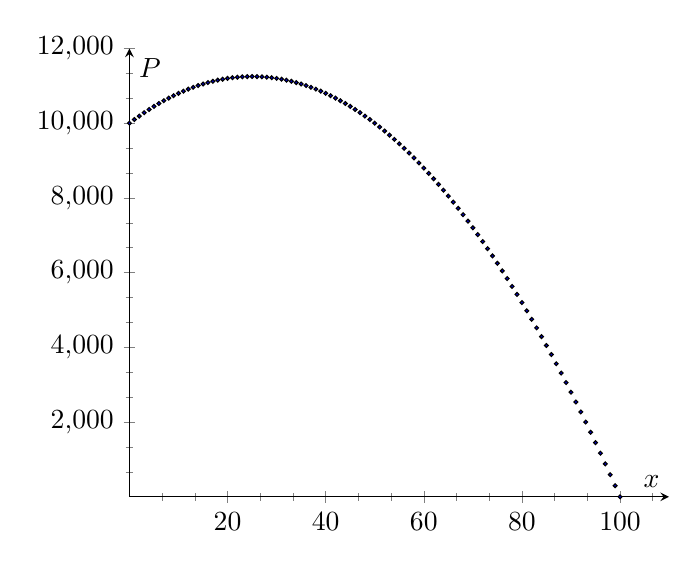
\begin{tikzpicture}
\begin{axis}[
	axis lines=middle,
	xmin=0, xmax = 110,
	ymin=0, ymax = 12000,
	xlabel={$x$}, ylabel={$P$},
	minor x tick num = {2},
	minor y tick num = {2},
	scaled ticks=false,
	yticklabel style={
		anchor = east,
		/pgf/number format/precision=0,
		/pgf/number format/fixed,
		/pgf/number format/fixed zerofill,
	},
]
%	\pgfplotsset{tick style={very thin,gray}}
    \addplot+[
    		mark=*,
		/tikz/fill=black,
		/tikz/color=black,
		/tikz/draw=black,
		/tikz/mark size={0.7},
    		only marks,
		domain=0:100,
		samples at={0,...,100}]
        {-2*x^2+100*x+10000};
\end{axis}
%\draw [dashed, thick] (25,0) -- (25,11500);
\end{tikzpicture}
\end{center}

}
	\end{enumerate}

\pagebreak
\item Currently, the average annual rate of interest on Vanguard's VBLTX (long-term bond index fund) is 7.67\%.\footnote{The average is taken over all the years that Vanguard has had this fund available for customers to invest in---that is, since March 1994. You can see the return rates for some of Vanguard's other mutual funds here: \texttt{https://investor.vanguard.com/mutual-funds/vanguard-mutual-funds-list}. The returns on some of their funds are lower than those on VBLTX, and others are higher.}
	\begin{enumerate}[label=\textbf{(\alph*)}]
	\item Suppose that you invest \$5,500 at one time this year in VBLTX, and that you stop contributing to this account afterward. If interest is compounded annually, and if the annual rate of interest stays fixed at 7.67\% per year, how much money will you have in that account forty years from now? (See Example 8 on Page 39.)

\sol{
You will have $\$5,500\cdot1.0767^{40}\approx\$105,718.55$ in the account at the end of forty years.
}

	\item Suppose that you wait ten years before investing your \$5,500. How much money will you have forty years from now in that case? (That is, how much will you have thirty years after you start investing?)
	
\sol{
If you wait 10 years before making your deposit, you will have $\$5,500\cdot1.0767^{40}\approx\$50,489.85$ in the account forty years from now---less than half of what you would have had if you'd made that initial deposit now.
}

	\item Suppose that beginning now, you invest \$5,500 per year in VBLTX for the next fifteen years (you deposit a total of fifteen times). How much money will you deposit over that period of time? (Do not compute interest yet.) If the interest rate remains fixed at 7.67\% and interest is compounded annually, compute the interest to find out how much money will be in your account at the end of the fifteenth year.
	
	Hint: The amount of money in your account will be the sum of fifteen terms:
	\begin{equation*}
	\sum^{15}_{i=1}5500\cdot1.0767^i=
	\underbrace{5500\cdot1.0767^1}_{\text{last deposit's contribution}}+
	5500\cdot1.0767^2+
	\cdots+
	5500\cdot1.0767^{14}+
	\underbrace{5500\cdot1.0767^{15}}_{\text{first deposit's contribution}}.
	\end{equation*}
	You might find a tool like WolframAlpha useful in computing this sum; use this example as a template:\\ \verb#http://www.wolframalpha.com/input/?i=%5Csum_%7Bi%3D0%7D%5E%7B20%7D+43*1.06%5Ei#, and change the numbers in it to obtain the sum above (the sum is under the ``Decimal Form'' heading).
	
\sol{
Over the next fifteen years, you will deposit $\$5,500\cdot15=\$82,500$ into the account, and will end up with ${\displaystyle \sum^{15}_{i=1}\$5,500\cdot1.0767^i\approx\$156,720.33}$ in the account at the end of those fifteen years.
}

	\item Continuing the scenario in part (c), suppose that you never make another contribution to that account after those first fifteen years go by, but that the interest rate remains fixed at the same rate of 7.67\% and compounds annually for the next thirty years after. How much will be in that account after those next thirty years have passed?
	
\sol{
Thirty years after you make your final deposit, the amount in the account will be $\$ 156,720.33\cdot1.0767^{30}\approx\$1,438,690.00$. Note that the interest generated on this principal alone will be $0.0767\cdot\$1,438,690.00\approx\$110,347.52$ per year, which I think is a pretty decent retirement salary.
}

	\item Suppose that your friend never thinks very much about his retirement now, and after his mid-life crisis in fifteen years, he begins to invest \$5,500 per year in VBLTX, with the same fixed 7.67\% rate of annually compounded interest, for the next thirty years after. How much money will he deposit in total? How much money will be in his account forty-five years from now, when you are both ready to retire? (Similar Hint: The total amount in his account at that time will be the sum of thirty terms---do this with WolframAlpha like you did part (c).)\footnote{I hope that doing this problem makes you think about how important it is to begin investing early. The interest on the student loans you pay won't be compounding for the rest of your life, but the interest your earn on your savings will---and, to boot, yearly IRA contributions are currently limited by U.S.\ law (to \$5,500 per year for people in your instructor's age and income bracket), making it truly impossible to catch up in the future if you fall behind now. So, learn more about IRAs here: \texttt{http://money.cnn.com/retirement/guide/IRA\_Basics.moneymag/index.htm}, and begin investing while you're young (:}

\sol{
Your friend will deposit $\$5,500\cdot30=\$165,000$ in total---exactly twice as much as you do---and will end up with ${\displaystyle \sum_{i=1}^{30}\$5,500\cdot1.0767^i\approx\$631,558.95}$, less than half (43\%) as much as you will.
}

	\end{enumerate}
	
\pagebreak

\item Recall the quadratic function that you found in Problem 1, part (a) to describe the production of an oil field.
	\begin{enumerate}[label=\textbf{(\alph*)}]
	\item Use Equation (10) on Page 59, or Equation 16 on Page 71 (your choice\footnote{Your answer will be the same no matter which equation you choose; Example 11 on Page 72 makes it clear why this is.}) to write the slope-predictor function $m$ of $P$.
	
\sol{The slope-predictor function for the parabola $y=ax^2+bx+c$ is $m(x)=2ax+b$. Thus, for our specific parabola, the slope predictor is $m(x)=-2(2)x+100=-4x+100$.
}	
	
	\item For which value of $x$ is the tangent line to the parabola $P$ horizontal? (Set $m(x)$ from part (a) equal to zero, and solve for $x$.) Does this agree with the maximum that you found in Problem 1, part (c)?
	
\sol{The line tangent to $P$ at the point $x$ is horizontal when $m(x)=0$. For our case, that happens when $-4x+100=0$, or when $x=25$. This does agree with the maximum that we found in Problem 1 (and if your answer here did not agree, then this should have been your reality check!).
}	
	
	\item On the same graph that you made for Problem 1, please add the plot of the line $m(x)$. Note that when $m(x)>0$, the slope of the line tangent to the parabola $P(x)$ is also positive---we say here that $P$ is \emph{increasing}, and conversely, we say that $P(x)$ is \emph{decreasing} when $m(x)<0$. Can you see this on the graph of $P$?

\sol{Note that I was asking here for the plot of $m(x)$---NOT of the tangent lines themselves. See the plot below.

\begin{center}
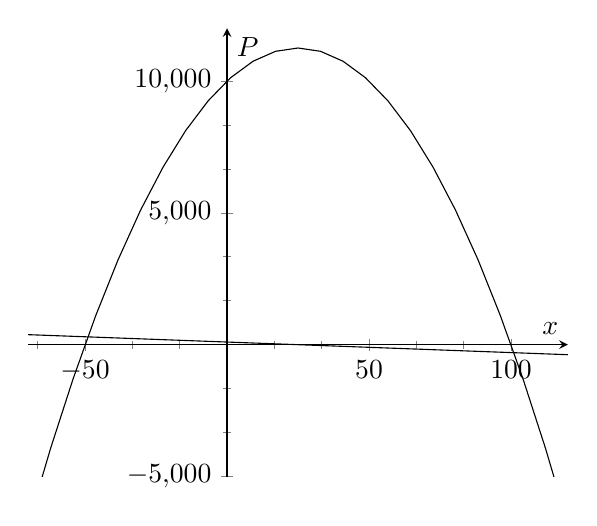
\begin{tikzpicture}
\begin{axis}[
	axis lines=middle,
	xmin=-70, xmax = 120,
	ymin=-5000, ymax = 12000,
	xlabel={$x$}, ylabel={$P$},
	minor x tick num = {2},
	minor y tick num = {2},
	scaled ticks=false,
	yticklabel style={
		anchor = east,
		/pgf/number format/precision=0,
		/pgf/number format/fixed,
		/pgf/number format/fixed zerofill,
	},
]
%	\pgfplotsset{tick style={very thin,gray}}
    \addplot[domain=-70:120]{-2*x^2+100*x+10000};
    \addplot[domain=-70:120]{-4*x+100};
    
\end{axis}
%\draw [dashed, thick] (25,0) -- (25,11500);
\end{tikzpicture}
\end{center}


}

	\item What do you think could be a good general rule for where a local maximum or minimum value of a function $f(x)$ occurs? In your answer, please mention the slope $m(x)$ of the line tangent to $f$ at $x$. (Hint: Think of a function's local maximum as a point where that function ceases to increase, and begins to decrease; conversely, think of a function's local minimum as a point where that function ceases to decrease, and begins to increase.) This answer is just supposed to be an informed guess on your part, and you will receive full credit as long as your answer makes sense---so please do not spend a lot of time looking up any general theorems or statements of this kind, unless you just cannot stop yourself. We will cover this topic in class shortly.
	
\sol{Based on what we've seen for the parabola case, a good guess at a general rule could be that an extremum of a function occurs when the tangent line has slope zero---that is, when $m(x)=0$. (When a function increases, $m(x)$ is positive; when it decreases, $m(x)$ is negative---thus, $m(x)$ will be zero at exactly the point where function ceases to increase and begins to decrease---that is, at the local maximum. A similar argument holds for local minima.)
}
	
	\end{enumerate}


\end{enumerate}

\end{document}